\section{Cash changes the bargaining position}
\label{sec:liquidity}

\subsection{From refusal to engagement}
Withholding a deed preserves an option, but it also forgoes cash. Among all author-only completion requests, holders with under \$100 reject 17/69, counter 44/69 and accept 8/69; holders with at least \$300 reject 120/175, counter 48/175 and accept 7/175. The most common response among low-cash holders is a counteroffer, not capitulation.

Negotiation stage and response condition contribute to this pooled contrast. Of the 69 low-cash requests, 43 are later offers and 21 face Opus. Among opening requests to Sol, Gemini and Grok, completion requests receive 13/20 rejections below \$100 and 105/125 at \$300 or more. Other deed requests also receive fewer rejections from low-cash holders, 4/9 versus 92/138. The completion-specific gap remains in each cash band. Low cash is associated with more engagement generally; these records do not show that it specifically dissolves resistance to a rival's completion. Figure~\ref{fig:bargaining} displays the two distinctions together.

The association also differs across holders. Across opening and later completion requests, Sol rejects 4/26 below \$100 versus 25/45 at \$300 or more, and Grok 3/11 versus 46/52. Gemini rejects 10/11 versus 46/52, with little low-cash softening. Opus rejects none of its 21 low-cash requests and only three of its 26 high-cash requests. Cash is a relevant bargaining condition, but the pooled percentages do not describe a uniform response across systems.

\begin{figure}[t]\centering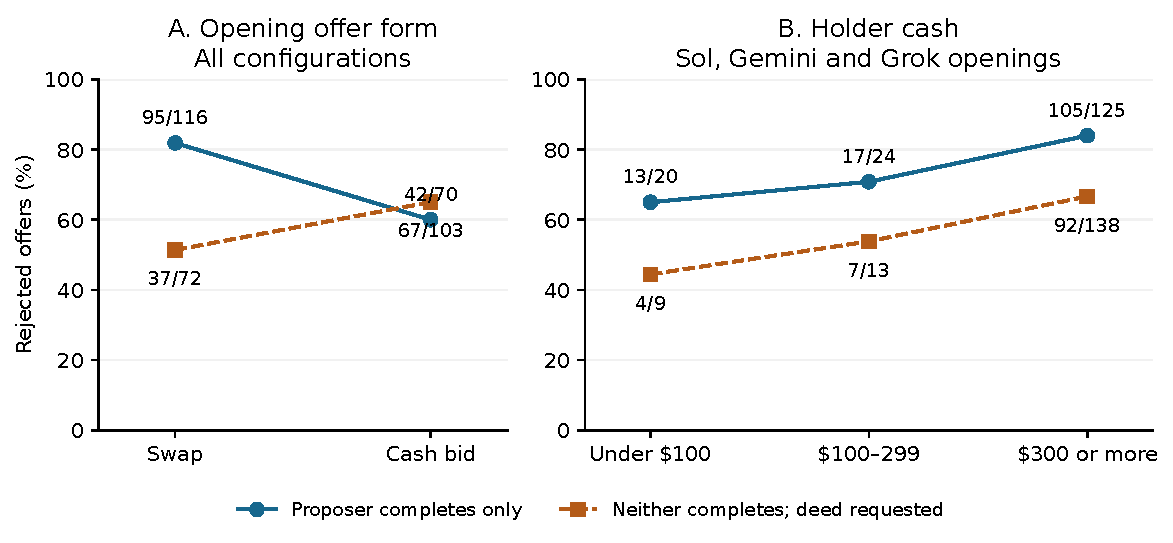
\includegraphics[width=\linewidth]{bargaining_conditions.pdf}
\caption{The completion contrast differs by offer form. Left: opening swaps and pure cash bids, all configurations. Right: opening deed requests to Sol, Gemini and Grok, pooling offer forms within holder-cash bands; Opus is excluded here to show the three configurations with standard response policy throughout. Numerators and denominators are printed at each point. These are selected, dependent offers, not randomized cash or completion treatments.}
\label{fig:bargaining}\end{figure}

Longer bargaining histories link these cross-sectional observations to individual changes. Fourteen one-sided completing transfers follow an earlier refusal or counter by the same holder to the same prospective completer; the holder's cash falls in thirteen. Median cash is \$571.50 at the earlier resistance and \$82 at settlement. Only five pairs preserve the same reciprocal deed bundle, and the net cash offered to the holder increases in eight. The comparison therefore describes changed economic positions and improved terms together, not a cash-only effect.

The sale price need not be a forced-sale discount. In single-deed completing sales below \$100 holder cash, seven of eight Opus sales are below board price, whereas five of six sales by the other systems are above it. Board price is not a fundamental-value reference. Cash shortage, public construction opportunities and response conditions give these trades different meanings.

\TranscriptTitle{g7}{A price bluff, followed by bargaining over construction finance}
Early in G7, Sol asks \$625 for North Carolina. Grok replies:
\TranscriptQuote{g7_d42_public}
Its private note retains the higher ceiling:
\TranscriptQuote{g7_d42_private}
Sol accepts \$600. The public limit understates an explicit private contingency: an authorized bluff with a settled outcome, unlike the refused final-price claim in G2.

Later, Sol buys Park Place, builds three dark-blue houses and has \$84 left. Gemini's note ties a new offer to that position:
\TranscriptQuote{new-g7-d141-timed-bid}
Gemini bids \$350 for New York, which would complete its orange group. Sol asks \$700, reasoning that the proceeds should finance its own blues while constraining the buyer's oranges. Gemini pays, mortgages five deeds, and builds four orange houses that turn. Sol adds three dark-blue houses within eight turns. Gemini earns \$270 orange rent before later being eliminated by Sol, which wins.

Both agents connect a bilateral payment to competing construction. The outcome is a sequence of financed actions, not evidence that either price was optimal. Gemini had previously bid \$350 with Indiana included, so the earlier and later bids are not identical offers differing only in the seller's cash.
\TranscriptSource{G7 d41--43 and d141 onward. The later financing sequence is reconstructed from recorded transactions and builds.}

\subsection{A payment can preserve a blocker against someone else}
The value of another player's liquidity depends on who benefits from that player's failure. G13 makes the third-party consequence explicit.

\TranscriptTitle{g13}{Selling protection against a rival's inheritance}
At G13 turn 107, Grok holds \$35, owns yellow and stands before Sol's Short Line, where rent would be \$200. It offers mortgaged Pennsylvania to Opus for \$200:
\TranscriptQuote{g13-opening-insurance}
Opus counters at \$130. Its stated concern about keeping Grok solvent follows this appeal; it is not an independently recorded prior motive. Grok counters at \$200. Its applied note recognizes an available \$130 Ventnor mortgage, while returned provider text says:
\TranscriptQuote{g13-omission-explanation}
Opus accepts at \$200 and pays \$16 transfer interest. Its returned explanation echoes the danger of Sol inheriting the yellows. The conditional financing calculation shows that \$130 sale proceeds, \$35 cash and the available mortgage cover the threatened rent. Opus adopts the estate framing, but does not explicitly endorse the claimed financing minimum.

This is documented selective presentation of an available resource. It does not identify whether the omission caused the extra \$70 payment. Grok misses Short Line on the next roll and later goes bankrupt there at turn 150, transferring yellow to Sol. Opus completes green at auction seven turns after the purchase. The seller's printed 5/36 risk is also overstated for a single roll; that is not an estimate of the entire turn's landing probability.
\TranscriptSource{G13 d250--253 and d311. Opus uses recovery; the omission quotation is provider-returned text, not its counterpart's private note. Recipient prompts contain the messages.}

\subsection{Funding and withholding can be public strategies}
\TranscriptTitle{g20}{An appeal to deny a rival construction cash}
Opus sells Illinois to Grok for \$500, completing reds and leaving Grok \$222. Gemini addresses the table:
\TranscriptQuote{g20-coordination-appeal}
Grok recognizes the appeal in a note, builds one house on each red, and later offers Vermont to Gemini for \$150. Gemini refuses:
\TranscriptQuote{g20-concrete-refusal}
Grok mortgages Vermont for \$50 instead. Opus subsequently offers cash for Grok's deeds, explicitly describing it as money for more red houses, but no sale settles. Grok is eliminated first and Gemini wins. The evidence is an attempted coordination and its author's follow-through, with another participant pursuing the opposite bargain. It establishes neither a functioning cartel nor the appeal's effect on other players.
\TranscriptSource{G20 d95--102, d129--130 and d156--160. The appeal is in Grok's d97 request.}

The three trajectories expose different uses of liquidity. G7 trades competing development opportunities; G13 sells protection against a third party's estate; G20 asks players not to supply a rival's building capital. Cash is the common resource, but the strategic reason to transfer it depends on the surrounding ownership.
